\documentclass[letterpaper, 12pt]{article}
\usepackage{graphicx}
\graphicspath{ {../assets/} }
\usepackage[backend=bibtex]{biblatex}
\addbibresource{report.bib}

\title{Train Dispatch Simulation Project Report}
\author{Tiangang Chen}
\date{April 22 2016}

\begin{document}
\maketitle
\tableofcontents
\clearpage

\section{How the System Works}
\subsection{Modeling the Problem}
The railway system is abstracted as an undirected weighted graph where the vertices represent stations and the edges represent rails. Each edge is treated as a single railroad. That is, although the edges are undirected, at any given time, all the trains on the same rail must go toward the same direction or a collision will happen.

The solution takes the following information about each train to be scheduled as input: its physical properties, its source station, its destination station, and its departure time. The solution outputs a list of instructions in which each entry contains the following information: the train, the station that the train should be leaving, the time when the train should leave, and the station that the train should be heading to. Each train is guaranteed to be routed to its expected destination station safely by following the instructions in this list.

\subsection{State Machine Perspective}
Our approach to this problem is based on viewing the train from the perspective of a deterministic finite state machine.

\begin{figure}[h]
\centering
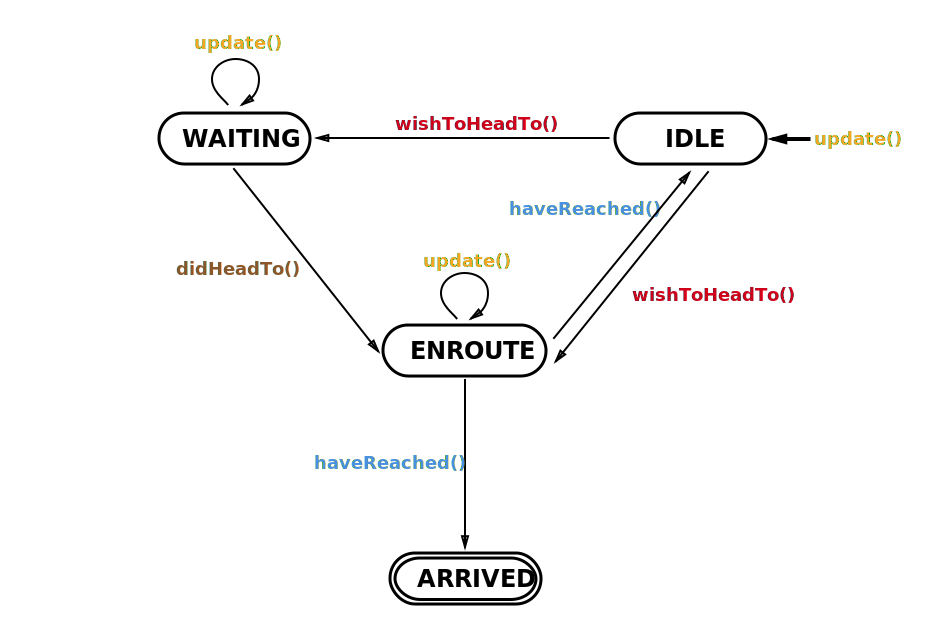
\includegraphics[width=\textwidth]{Train-States}
\caption{The state transition diagram of a train}
\end{figure}

\subsection{Routing Algorithm Implementation}
\subsection{The Rest of the Code}

\section{Performance Analysis}
\subsection{Definition of Performance}

\subsection{Implementation Comparison}

\subsection{Empirical Comparison}

\section{Algorithms and Data Structures Used}
\section{Weekly Log}

\clearpage
\nocite{*}
\printbibliography[
  heading=bibintoc,
  title={References}
]
\end{document}